\documentclass{apcalc}
\title{Unit 1: Limits and Continuity}
\author{Paul Wang}
\date{November 2026}
\volume{Study Guide 1 of 10 (topics 1.1--1.16)}
\shorttitle{Unit 1 --- Study Guide}
\begin{document}
\maketitle

\begin{abstract}
Limits are the language of the whole course: the derivative, the definite integral and every series test are limits. Unit 1 carries 5--10\% of the multiple-choice section and appears in almost every free-response question as a justification (``$f$ is continuous because \dots'', ``by the Intermediate Value Theorem \dots''). This guide states the unit in sixteen numbered rules (R1.1--R1.16) across six sections, works one example per idea, and flags the traps that cost points. The \emph{Unit 1 Practice Set} uses the same section numbers, so every missed item points back here.
\end{abstract}
\keywords{limit, one-sided limit, squeeze theorem, continuity, removable discontinuity, vertical and horizontal asymptotes, end behavior, Intermediate Value Theorem.}

\section*{Router: what to do when you see a limit}
\begin{router}
$\lim_{x\to a} f(x)$ and $f$ is continuous at $a$ & substitute $x=a$ & R1.4 \\
substitution gives $\tfrac{0}{0}$ with polynomials or roots & factor and cancel, or multiply by the conjugate & R1.5 \\
$\tfrac{0}{0}$ with $\sin$, $1-\cos$ & rewrite toward $\frac{\sin u}{u}\to1$, $\frac{1-\cos u}{u}\to0$ & R1.6 \\
a bounded oscillating factor ($\sin\frac1x$, $\cos x^2$) & squeeze between two functions with the same limit & R1.7 \\
substitution gives $\tfrac{c}{0}$ with $c\neq0$ & infinite limit: check the sign on each side & R1.11 \\
$x\to\pm\infty$ with a rational function & compare degrees (leading terms) & R1.12 \\
$x\to\pm\infty$ with $\sqrt{x^2+\dots}$ & factor $|x|$ out of the root; watch the sign as $x\to-\infty$ & R1.13 \\
a piecewise function and ``continuous at $a$'' & three conditions; match one-sided limits to $f(a)$ & R1.8, R1.10 \\
``must there be a value $c$ with $f(c)=k$?'' & Intermediate Value Theorem: continuity on $[a,b]$ first & R1.15 \\
a limit you cannot simplify (Unit 4) & L'H\^opital's rule, after confirming $\tfrac00$ or $\tfrac{\infty}{\infty}$ & R4.9 \\
\end{router}

\section{What a limit is (1.1--1.4)}

\begin{rulebox}{R1.1}{Definition in words}
$\lim_{x\to a} f(x)=L$ means $f(x)$ can be made as close to $L$ as we like by taking $x$ close enough to $a$, \emph{with $x\neq a$}. The value $f(a)$ plays no role: it may differ from $L$ or not exist at all.
\end{rulebox}

\begin{rulebox}{R1.2}{One-sided limits}
$\lim_{x\to a^-}$ uses $x<a$ only; $\lim_{x\to a^+}$ uses $x>a$ only. The two-sided limit exists if and only if both one-sided limits exist and are equal. A limit that grows without bound \emph{does not exist} as a number; writing $=\infty$ describes how it fails.
\end{rulebox}

\begin{rulebox}{R1.3}{Reading graphs and tables}
From a graph, follow the curve toward $x=a$ from each side and read the height it approaches; ignore any isolated dot at $x=a$. From a table, look at the trend of $f(x)$ as $x$ approaches $a$ from both sides; a table suggests a limit but never proves one.
\end{rulebox}

\begin{example}{reading a graph}
\begin{center}
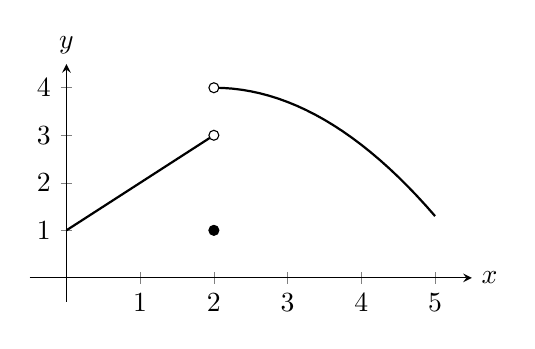
\begin{tikzpicture}
\begin{axis}[width=7.2cm,height=4.6cm,axis lines=middle,xmin=-0.5,xmax=5.5,ymin=-0.5,ymax=4.5,xtick={1,2,3,4,5},ytick={1,2,3,4},xlabel={$x$},ylabel={$y$},every axis x label/.style={at={(ticklabel* cs:1)},anchor=west},every axis y label/.style={at={(ticklabel* cs:1)},anchor=south}]
\addplot[thick,domain=0:2]{x+1};
\addplot[thick,domain=2:5]{4-0.3*(x-2)^2};
\addplot[only marks,mark=*,mark size=1.8pt] coordinates{(2,1)};
\addplot[only marks,mark=*,mark size=1.8pt,mark options={fill=white}] coordinates{(2,3) (2,4)};
\end{axis}
\end{tikzpicture}
\end{center}
For the graph above, $\lim_{x\to2^-}f(x)=3$, $\lim_{x\to2^+}f(x)=4$, so $\lim_{x\to2}f(x)$ does not exist; $f(2)=1$ (the isolated solid dot). \answer{the two one-sided limits differ, so the limit fails to exist even though $f(2)$ is defined.}
\end{example}

\begin{rulebox}{R1.4}{Limit laws and direct substitution}
Limits respect sums, differences, constant multiples, products, quotients (nonzero denominator limit) and powers. Polynomials, rational functions (where defined), roots, exponentials, logarithms and trig functions are continuous on their domains, so for these \emph{substitute first}: if $f$ is continuous at $a$, then $\lim_{x\to a}f(x)=f(a)$.
\end{rulebox}

\section{Evaluating limits algebraically (1.5--1.7)}

\begin{rulebox}{R1.5}{Indeterminate $\tfrac00$: factor, cancel, rationalize}
$\tfrac00$ is a signal, not an answer. Factor and cancel the common factor $(x-a)$; for square roots multiply top and bottom by the conjugate; for complex fractions combine over a common denominator. Then substitute again.
\end{rulebox}

\begin{example}{conjugate}
$\displaystyle\lim_{x\to9}\frac{\sqrt{x}-3}{x-9}=\lim_{x\to9}\frac{(\sqrt{x}-3)(\sqrt{x}+3)}{(x-9)(\sqrt{x}+3)}=\lim_{x\to9}\frac{1}{\sqrt{x}+3}=\frac16.$
(Factoring $x-9=(\sqrt x-3)(\sqrt x+3)$ gives the same result in one line.)
\end{example}

\begin{rulebox}{R1.6}{The two special trig limits (radians)}
\[\lim_{u\to0}\frac{\sin u}{u}=1,\qquad \lim_{u\to0}\frac{1-\cos u}{u}=0.\]
Make the argument and the denominator match: $\displaystyle\lim_{x\to0}\frac{\sin 5x}{3x}=\frac53\cdot\lim_{x\to0}\frac{\sin5x}{5x}=\frac53$, and $\displaystyle\lim_{x\to0}\frac{\tan x}{x}=\lim\frac{\sin x}{x}\cdot\frac1{\cos x}=1$.
\end{rulebox}

\begin{trap}
$\lim_{x\to\infty}\frac{\sin x}{x}=0$, not 1: the special limit needs the argument going to 0. Here $|\sin x|\le1$ while $x\to\infty$, so the squeeze theorem gives 0.
\end{trap}

\section{The squeeze theorem (1.8--1.9)}

\begin{rulebox}{R1.7}{Squeeze theorem}
If $g(x)\le f(x)\le h(x)$ near $a$ (except possibly at $a$) and $\lim g=\lim h=L$, then $\lim_{x\to a}f(x)=L$. Typical use: a bounded factor times something going to 0, e.g.\ $-x^2\le x^2\sin\frac1x\le x^2$, so $\lim_{x\to0}x^2\sin\frac1x=0$.
\end{rulebox}

\begin{frqtip}
To use the squeeze theorem on a free-response question, state both inequalities, state that both outer limits equal $L$, and name the theorem. Tables of bounds (``$g(x)\le f(x)\le h(x)$ for all $x$'') are common in Part A.
\end{frqtip}

\section{Continuity and discontinuities (1.10--1.13)}

\begin{rulebox}{R1.8}{Continuity at a point: three conditions}
$f$ is continuous at $x=a$ when (1) $f(a)$ is defined, (2) $\lim_{x\to a}f(x)$ exists, and (3) $\lim_{x\to a}f(x)=f(a)$. On the exam, write all three for a piecewise function: compute both one-sided limits and $f(a)$, and show they agree.
\end{rulebox}

\begin{rulebox}{R1.9}{Types of discontinuity}
\textbf{Removable} (a hole): the limit exists but $f(a)$ is undefined or $\neq$ the limit. \textbf{Jump}: both one-sided limits exist but differ. \textbf{Infinite}: a one-sided limit is $\pm\infty$ (a vertical asymptote). A rational function has a hole where a factor cancels and a vertical asymptote where a zero of the denominator survives cancellation.
\end{rulebox}

\begin{rulebox}{R1.10}{Making a piecewise function continuous}
Set the left-hand limit equal to the right-hand limit (and to $f(a)$). With two unknown constants, a second condition is needed; in Unit 2 it is usually differentiability (matching slopes).
\end{rulebox}

\begin{example}{choosing a constant}
$f(x)=\begin{cases}kx^2-1,&x<2\\ 3x+k,&x\ge2\end{cases}$. Continuity at 2: $4k-1=6+k$, so $k=\tfrac73$. \answer{$k=7/3$.}
\end{example}

\begin{example}{removing a discontinuity}
$g(x)=\dfrac{x^2-x-6}{x-3}$ for $x\neq3$. Since $\frac{(x-3)(x+2)}{x-3}=x+2\to5$, defining $g(3)=5$ makes $g$ continuous at 3. \answer{$g(3)=5$.}
\end{example}

\section{Infinite limits and limits at infinity (1.14--1.15)}

\begin{rulebox}{R1.11}{Infinite limits and vertical asymptotes}
If substitution gives $\frac{c}{0}$ with $c\ne0$, the one-sided limits are $\pm\infty$. Find each sign from a sign check: $\lim_{x\to1^+}\frac{x+2}{x-1}=+\infty$ (numerator $3>0$, denominator small positive) and $\lim_{x\to1^-}=-\infty$. Then $x=1$ is a vertical asymptote.
\end{rulebox}

\begin{rulebox}{R1.12}{Rational functions at $\pm\infty$}
Compare degrees of numerator ($n$) and denominator ($d$). $n<d$: limit 0. $n=d$: ratio of leading coefficients. $n>d$: $\pm\infty$ (no horizontal asymptote). A horizontal asymptote $y=L$ means $\lim_{x\to\infty}f=L$ or $\lim_{x\to-\infty}f=L$.
\end{rulebox}

\begin{rulebox}{R1.13}{Roots, exponentials and dominance}
$\sqrt{x^2}=|x|$, so for $x\to-\infty$ write $\sqrt{x^2}=-x$: $\displaystyle\lim_{x\to-\infty}\frac{\sqrt{4x^2+1}}{x}=-2$ while the limit at $+\infty$ is $2$. Growth order as $x\to\infty$: $\ln x\ll x^p\ll e^x$ ($p>0$); the faster function dominates a quotient. And $e^{x}\to0$ as $x\to-\infty$.
\end{rulebox}

\begin{example}{two different horizontal asymptotes}
$f(x)=\dfrac{3x}{\sqrt{x^2+4}}$. For $x>0$, $\sqrt{x^2+4}=x\sqrt{1+4/x^2}$, so $f\to3$; for $x<0$, $\sqrt{x^2+4}=-x\sqrt{1+4/x^2}$, so $f\to-3$. \answer{asymptotes $y=3$ and $y=-3$.}
\end{example}

\section{The Intermediate Value Theorem (1.16)}

\begin{rulebox}{R1.14}{Continuity on intervals}
A function is continuous on $[a,b]$ if it is continuous at every interior point and one-sided continuous at the endpoints. Sums, products, quotients (nonzero denominators) and compositions of continuous functions are continuous. Differentiable implies continuous (Unit 2).
\end{rulebox}

\begin{rulebox}{R1.15}{Intermediate Value Theorem (IVT)}
If $f$ is continuous on $[a,b]$ and $k$ is between $f(a)$ and $f(b)$, then $f(c)=k$ for at least one $c$ in $(a,b)$ ($[a,b]$ if $k$ equals an endpoint value). The IVT guarantees existence, not uniqueness or location.
\end{rulebox}

\begin{rulebox}{R1.16}{IVT with tables}
Given a table for a continuous $f$, every time consecutive values cross $k$, the IVT guarantees a solution of $f(x)=k$ in that subinterval. Counting crossings gives the \emph{minimum} number of solutions.
\end{rulebox}

\begin{example}{a table and the IVT}
$f$ is continuous with $f(0)=2$, $f(1)=-1$, $f(3)=4$, $f(5)=1$. On $[0,5]$, $f(x)=0$ must have at least two solutions: one in $(0,1)$ (2 to $-1$) and one in $(1,3)$ ($-1$ to 4). From 4 to 1 the values never reach 0, so no third solution is guaranteed.
\answer{at least two.}
\end{example}

\begin{frqtip}
The scoring guide awards the IVT point only when the response says the function is \emph{continuous} (or differentiable), names the interval, and shows the target value lies between the endpoint values. Template: ``$f$ is differentiable, hence continuous, on $[1,3]$, and $f(1)=-1<0<4=f(3)$, so by the IVT there is a $c$ in $(1,3)$ with $f(c)=0$.''
\end{frqtip}

\section{Common errors}
\begin{itemize}
\item Reporting $f(a)$ as the limit for a piecewise or holed function (R1.1).
\item Stopping at $\tfrac00$ and calling the limit undefined (R1.5).
\item Forgetting $\sqrt{x^2}=|x|$ as $x\to-\infty$ (R1.13).
\item Citing the IVT without stating continuity (R1.15).
\item Calling every zero of the denominator a vertical asymptote: a canceled factor is a hole (R1.9).
\end{itemize}

\end{document}
